\subsection{Apparato B}

Dopo aver eseguito in maniera preliminare le misure richieste, abbiamo deciso di semplificare l'apparato per tenere sotto controllo le criticità descritte nella sezione precedente.

\subsubsection{Descrizione del circuito}

Il nuovo circuito segue lo schema in \autoref{disegno}.
\marginpar{Jack deve disegnare l'apparato B}
I segnali dei PMT vengono inviati ai discriminatori per ottenere i segnali logici e agli attenuatori per essere poi inviati all'ADC. I segnali logici attraversano un modulo di antiretrigger per poi essere usati come trigger di acquisizioni singole o per effettuare coincidenze. Una copia dei segnali finisce al contatore. Abbiamo usato il timer per far partire/fermare le acquisizioni come abbiamo fatto per l'apparato precedente.

\subsubsection{Problemi riscontrati}
\label{ref}
Dopo aver acceso l'apparato il bit stuck è scomparso e l'aumento di risoluzione ci ha permesso di notare un problema che era già presente nell'apparato precedente. Abbiamo iniziato a vedere uno sdoppiamento dello spettro, come evidenziato dalla \autoref{doppio}. 

\begin{figure}[h]
\centering
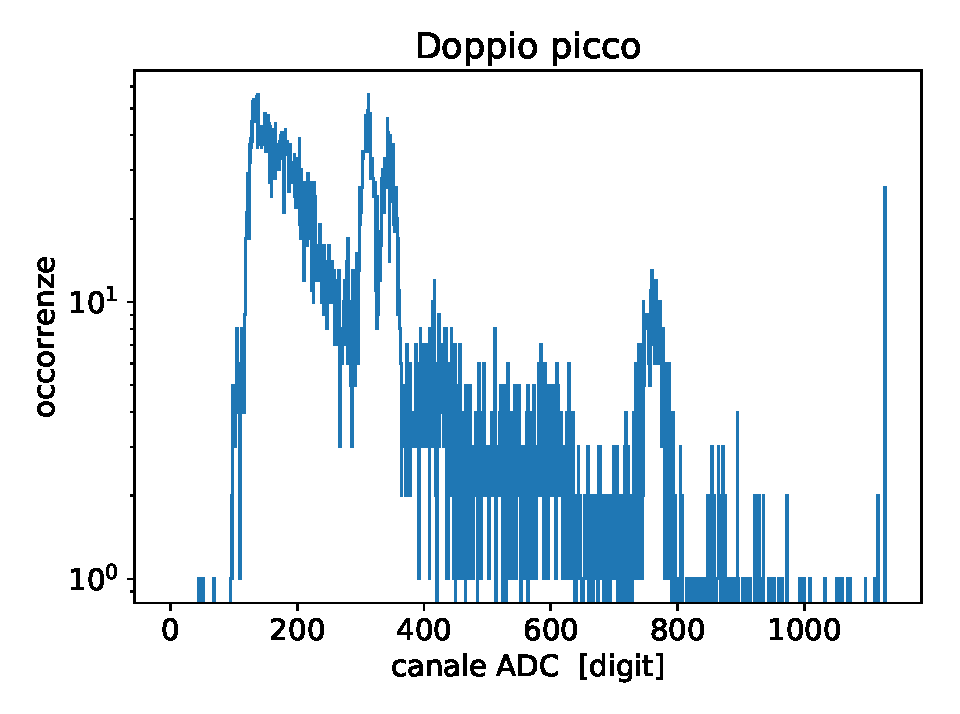
\includegraphics[width=20 em]{immagini/doppio}
\caption{Acquisizione in cui l'annichilazione presenta due picchi.}
\label{doppio}
\end{figure}

Tale problema non era visibile ad occhio nudo nelle precedenti acquisizioni, ma un fit eseguito in seguito ha mostrato la presenza di due gaussiane sovrapposte.

\marginpar{Mi pare che sia coincidenza/anticoincidenza (come detto subito dopo) che ci convince del doppio picco, non uno dei fit.
\texttt{Io mi riferivo a quella misura di stabilità in cui non si vedeva che i picchi erano 2}}

Abbiamo poi scoperto la causa del problema, ovvero il crosstalk.
Come mostra il grafico di Figura\autoref{sdoppio}, il doppio picco è la somma di quello osservato nelle acquisizioni in coincidenza con quello osservato in anticoincidenza. 

\begin{figure}[h]
\centering
\subfloat
{
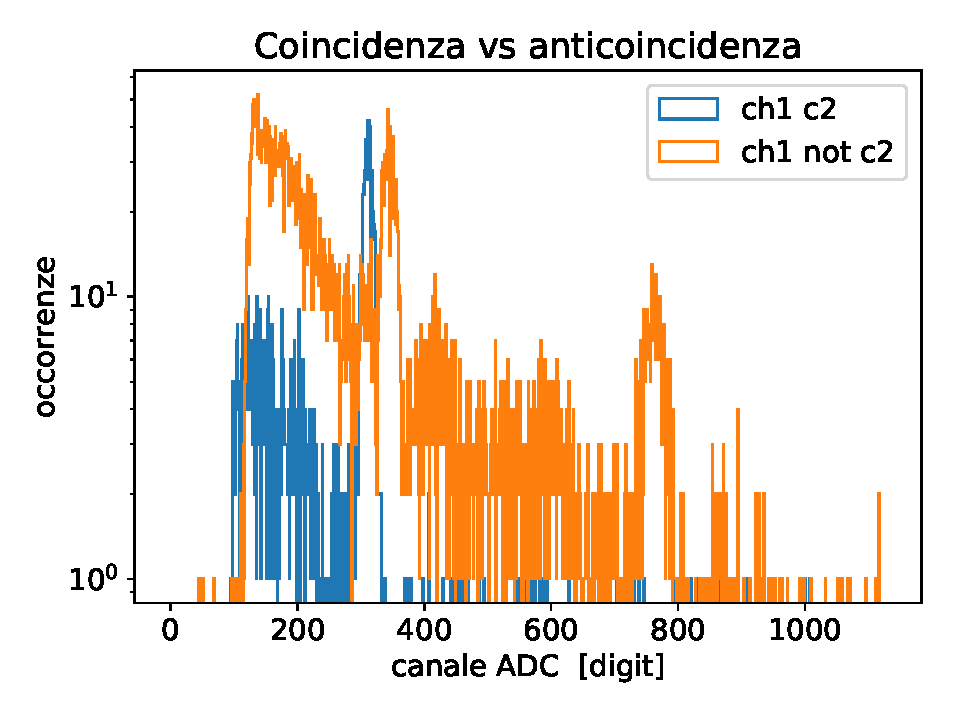
\includegraphics[width=18 em]{immagini/sdoppio}
\label{sdoppio}
}
\subfloat
{
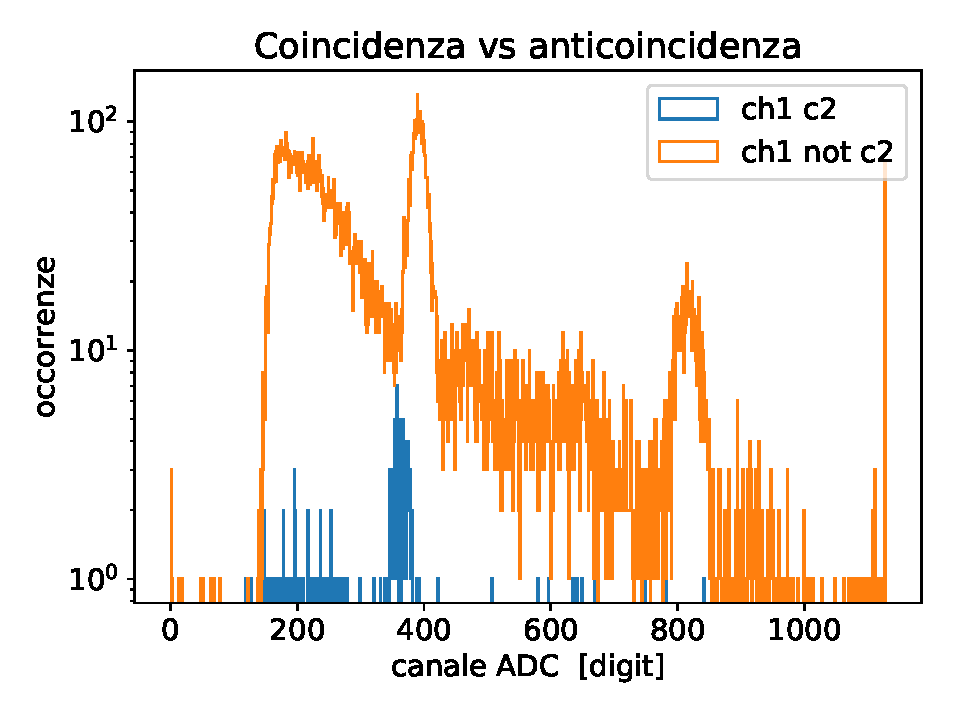
\includegraphics[width=18 em]{immagini/dist}
\label{dist}
}

\caption{A sinistra: rappresentazione di dell'acquisizione di \autoref{doppio} separando le coincidenze dalle anticoincidenze. \\
A destra: grafico della stessa misura in cui il PMT1 è vicino alla sorgente mentre il PMT2 è lontano dalla sorgente.}

\end{figure}

Siamo arrivati alla conclusione che si tratti di un crosstalk dal fatto che il picco in anticoincidenza coincide con quello delle acquisizioni singole. Inoltre abbiamo visto, aumentando la distanza di un PMT dalla sorgente, che il picco delle coincidenze si rimpicciolisce (perché ha meno eventi) e il picco in anticoincidenza tende ad assomigliare sempre di più a quello dell'acquisizione con canale singolo (Figura\autoref{dist}).
In seguito abbiamo provato che questo problema si riscontra anche quando i canali da analizzare non sono collegati ad ingressi adiacenti dell'ADC. Inspiegabilmente, il problema si è ripresentato solo a giorni alterni. 
